\documentclass[letterpaper, 10 pt, conference]{ieeeconf}
\IEEEoverridecommandlockouts
\overrideIEEEmargins

\usepackage{graphicx}
\usepackage{booktabs}
\usepackage{url}
\usepackage{listings}
\usepackage{amsmath}
\usepackage{amssymb}
\usepackage{balance}
\usepackage{xcolor}

\graphicspath{{figures/}}
\renewcommand{\ttdefault}{cmtt}
\lstset{
  basicstyle=\ttfamily\scriptsize,
  columns=fullflexible,
  keepspaces=true,
  frame=single,
  breaklines=true,
  showstringspaces=false
}

\title{\LARGE \bf
LAB2 Report: ROS Installation and TF-Based\ Two-Drone Trajectory Analysis
}

\author{Haoran Xiao\\Student No.: 24020036066}

\begin{document}
\maketitle
\thispagestyle{empty}
\pagestyle{empty}

\begin{abstract}
This report documents the completion of a ROS laboratory on installation, workspace configuration, node and topic inspection, TF broadcasting, TF lookup, visualization, and rigid-transformation analysis. The course material specifies Ubuntu 20.04 with ROS1 Noetic, while the available Lab1 virtual machine was Ubuntu 22.04.5 LTS with no native ROS installation. To preserve the required ROS1 environment without replacing the virtual machine, Docker was used to run the official OSRF ROS Noetic desktop image. The ROS1-compatible Lab2 package was selected at commit \texttt{609f31f} after the current repository tip was correctly identified as a ROS2 \texttt{ament\_cmake} package. The workspace compiled successfully, the static and moving two-drone scenes ran in rViz, the node/topic graph was inspected, and the relative trajectory was visualized in the AV1 frame. The measured mathematical result is that the relative trajectory lies on \(z-2y=1\) and is an ellipse with semi-axis lengths \(1/2\) and \(\sqrt{5}/2\). The evidence supports successful software-in-the-loop visualization and compilation; it does not establish physical-robot execution.
\end{abstract}

\section{INTRODUCTION AND OBJECTIVES}
\label{sec:introduction}
Robot Operating System (ROS) provides a communication and tooling layer for robotics applications. In a visual-navigation system, a single geometric object is commonly represented in several coordinate frames, such as a world frame, a vehicle body frame, and sensor frames. The ability to publish, inspect, and query these frame relationships is therefore a prerequisite for later navigation, estimation, and control laboratories.

This laboratory had four connected objectives. First, it required a working ROS environment and a catkin workspace. Second, it required inspection of ROS nodes, topics, launch files, and the rViz visualization pipeline. Third, it required implementation of two ROS1 nodes: one to publish the prescribed motion of two aerial vehicles through TF, and one to query a relative transform and draw the resulting trajectory. Finally, it required mathematical derivations using homogeneous transformations, rotation matrices, and quaternion identities.

The experiment was designed to connect implementation and theory. The code makes the two trajectories observable, while the coordinate-frame analysis explains why the trajectory of AV2 relative to AV1 is an ellipse on a slanted plane. This combination is relevant to later robotics projects because a program may compile while still using the wrong frame direction, and a visually plausible plot may still represent the wrong transform.

The expected outcome was a reproducible ROS1 workspace containing the Lab2 package, a successful catkin build, a static and dynamic rViz demonstration, a node/topic graph, a relative-frame visualization, and a report supported by traceable evidence.

\section{EXPERIMENTAL ENVIRONMENT}
\label{sec:environment}
\subsection{Required and Actual Environments}
The supplied Lab2 handout specifies Ubuntu 20.04 with ROS1 Noetic. The available Lab1 virtual machine was instead Ubuntu 22.04.5 LTS, and the initial checks showed that neither \texttt{/opt/ros} nor the ROS commands were present. Installing only \texttt{python3-rospkg} would not have installed a complete ROS distribution, so that route was not used.

The actual solution kept the existing virtual machine as the host and ran Ubuntu 20.04 with ROS Noetic inside the OSRF Docker image \texttt{osrf/ros:noetic-desktop-full}. This separated the host operating-system version from the ROS distribution required by the experiment. The container was launched with host networking, the X11 socket, the display variable, and a persistent workspace mount so that ROS nodes and rViz could run together.

\begin{table}[t]
\caption{Verified experimental environment.}
\label{tab:environment}
\centering
\footnotesize
\setlength{\tabcolsep}{2pt}
\begin{tabular}{p{0.32\columnwidth}p{0.58\columnwidth}}
\toprule
Item & Verified value \\
\midrule
Host OS & Ubuntu 22.04.5 LTS in the Lab1 virtual machine \\
Container image & \texttt{osrf/ros:noetic-desktop-full} \\
ROS distribution & ROS1 Noetic; \texttt{rosversion -d} returned \texttt{noetic} \\
Workspace & \texttt{/root/vnav\_ws} inside the container \\
Build system & \texttt{catkin\_tools}; linked devel space \\
Visualization & rViz and rqt\_graph through the container display \\
Source version & MIT-SPARK/VNAV-labs commit \texttt{609f31f} \\
Hardware & No physical robot or UAV was used; simulation/visualization only \\
\bottomrule
\end{tabular}
\end{table}

Figure~\ref{fig:docker} records the successful Docker smoke test. Figure~\ref{fig:image} records the Noetic image download, and Fig.~\ref{fig:rosworkspace} records the Noetic version and catkin workspace initialization. These figures establish the environment boundary used by the rest of the report.

\begin{figure}[t]
\centering
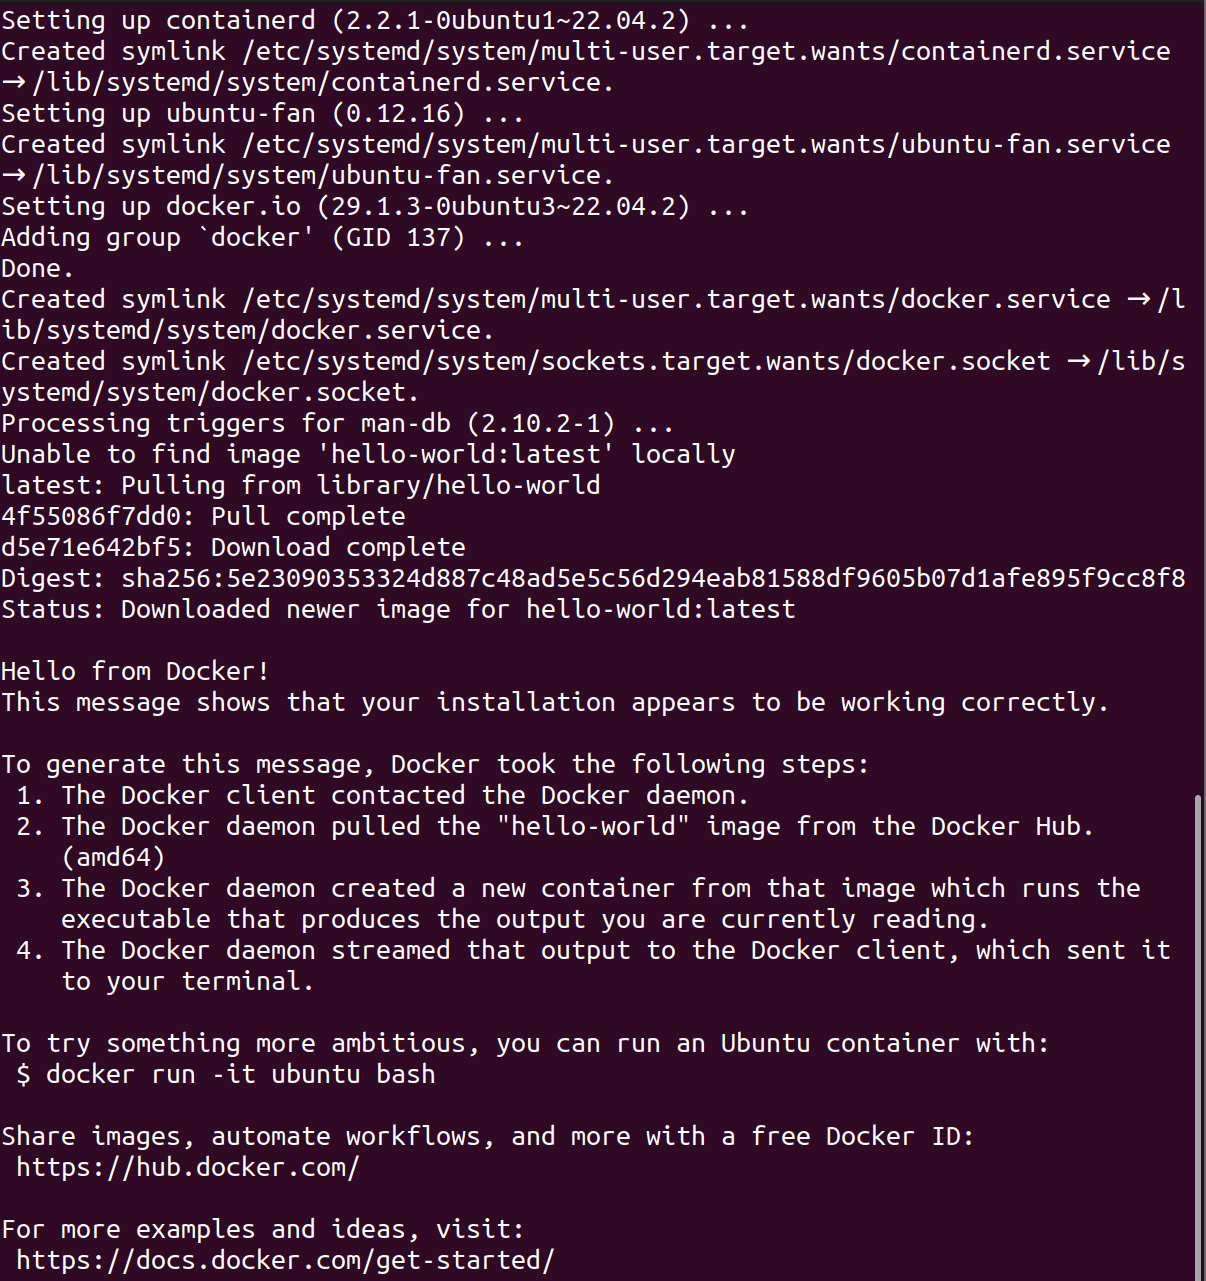
\includegraphics[width=\columnwidth,keepaspectratio]{01_docker_hello_world.png}
\caption{Docker smoke test returning ``Hello from Docker!'' on the Ubuntu 22.04 host.}
\label{fig:docker}
\end{figure}

\begin{figure}[t]
\centering
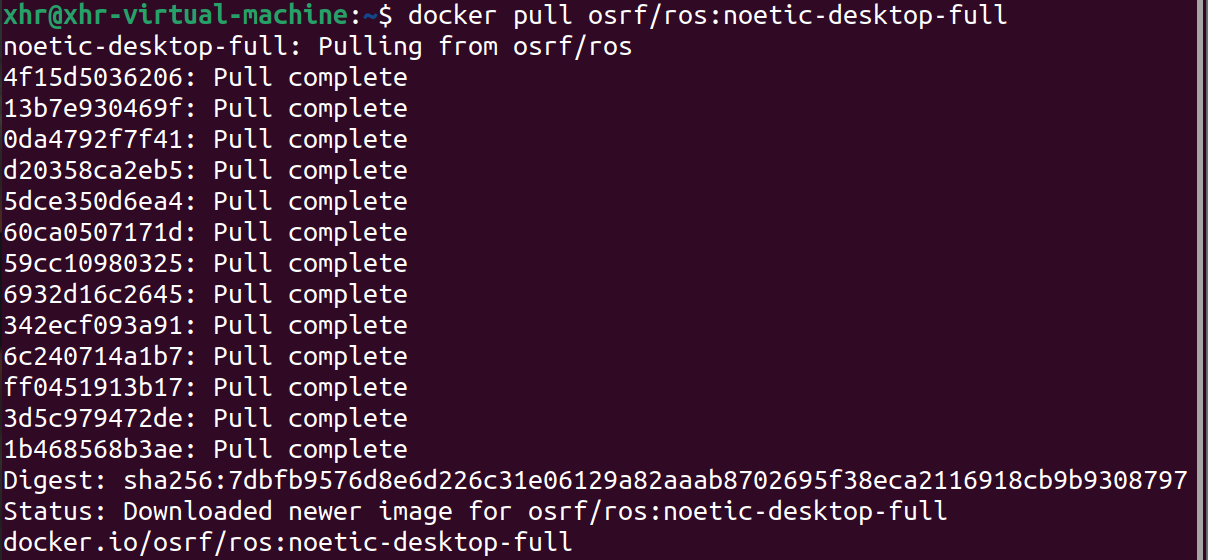
\includegraphics[width=\columnwidth,keepaspectratio]{03_ros_noetic_image.png}
\caption{Successful pull of the OSRF ROS Noetic desktop image.}
\label{fig:image}
\end{figure}

\begin{figure}[t]
\centering
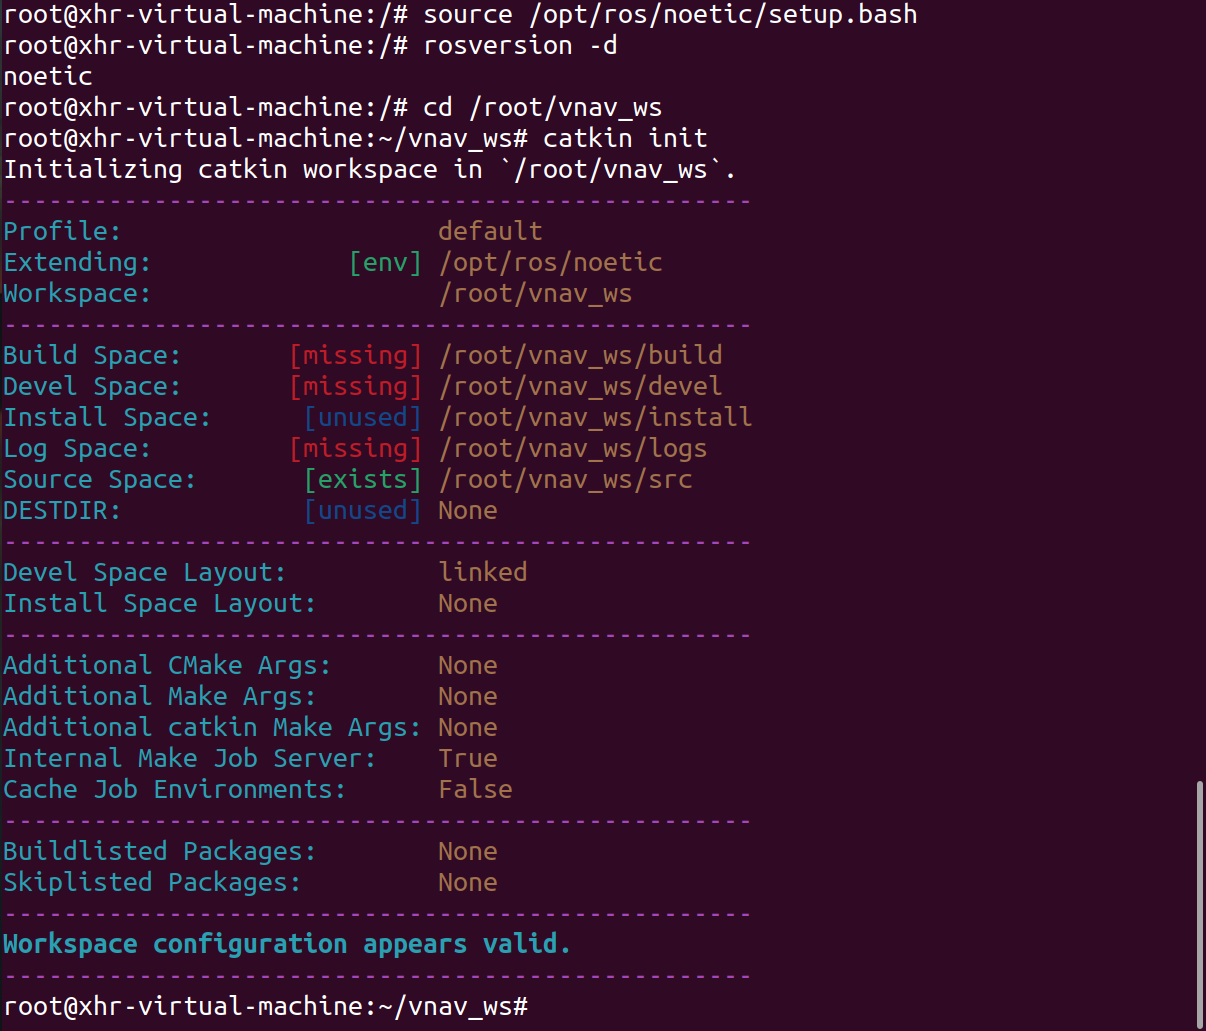
\includegraphics[width=\columnwidth,keepaspectratio]{04_workspace_init.png}
\caption{ROS Noetic version check and valid catkin workspace initialization.}
\label{fig:rosworkspace}
\end{figure}

\section{EXPERIMENTAL PLAN AND PROCESS}
\label{sec:process}
The experiment was executed as a sequence of independently checkable stages. Each stage had a distinct purpose and a visible success condition.

\subsection{Stage 1: Docker access and ROS image preparation}
The first input was the existing Ubuntu 22.04 virtual machine. Docker was installed and the user was added to the Docker group. The \texttt{hello-world} image verified communication among the Docker client, daemon, registry, and container runtime. The user-group check was then repeated after re-login; \texttt{id -nG} included \texttt{docker} and \texttt{docker ps} no longer returned a permission error. Figure~\ref{fig:dockerperm} is the corresponding access evidence. The Noetic desktop image was pulled only after this permission check succeeded.

\begin{figure}[t]
\centering
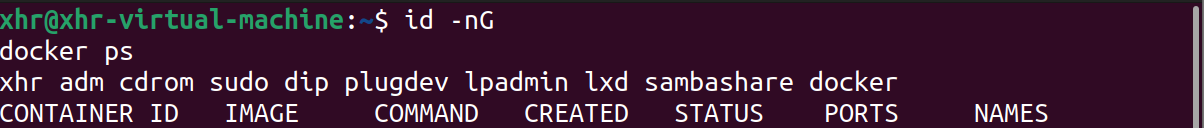
\includegraphics[width=\columnwidth,keepaspectratio]{02_docker_permission.png}
\caption{Non-root Docker access after the user-group update.}
\label{fig:dockerperm}
\end{figure}

\subsection{Stage 2: Workspace and source preparation}
Inside the container, the ROS environment was sourced and the workspace was initialized with \texttt{catkin init}. The package was cloned from \texttt{MIT-SPARK/VNAV-labs} and copied into \texttt{/root/vnav\_ws/src}. Figure~\ref{fig:package} shows the package structure, including \texttt{CMakeLists.txt}, \texttt{package.xml}, launch files, configuration files, meshes, and source code.

\begin{figure}[t]
\centering
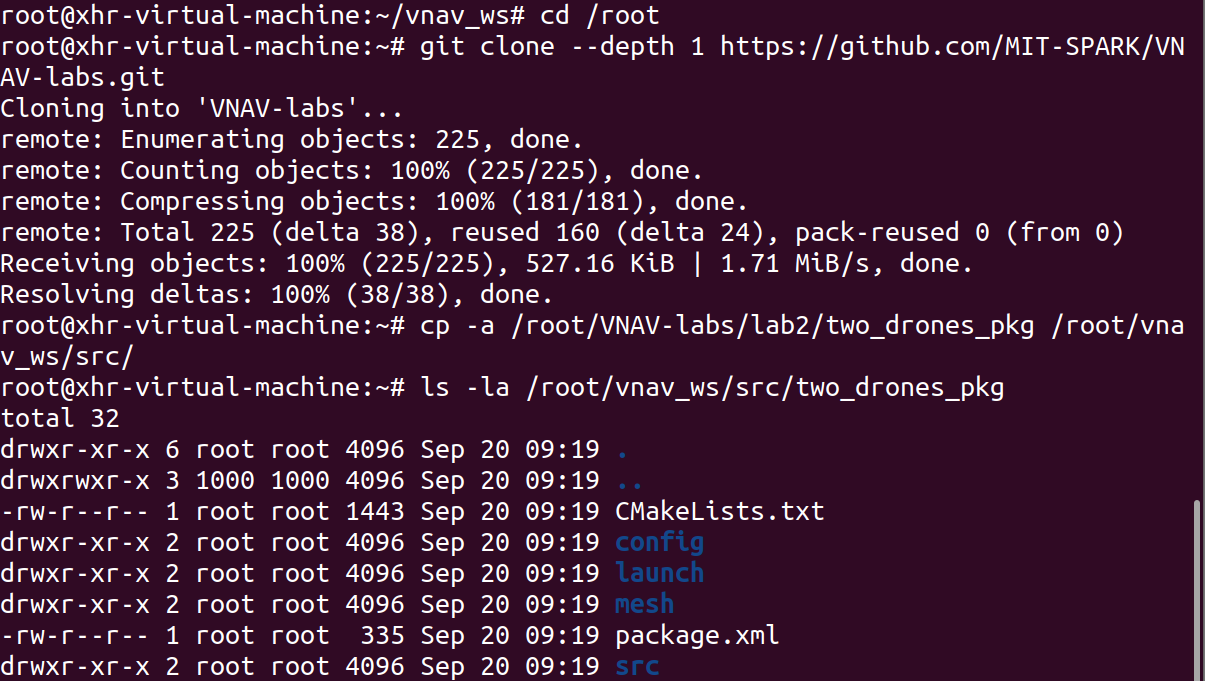
\includegraphics[width=\columnwidth,keepaspectratio]{05_package_copied.png}
\caption{The Lab2 package copied into the catkin source space.}
\label{fig:package}
\end{figure}

The first shallow clone used the current repository tip. Catkin reported that the package had an unsupported \texttt{ament\_cmake} build type, so it skipped the package rather than compiling it. This was a diagnostic result, not a successful build, and is retained in Fig.~\ref{fig:mismatch}. The full Git history was then fetched and the package history was inspected. Commits \texttt{2f199b4}, \texttt{04e9eba}, and \texttt{609f31f} used catkin, whereas \texttt{ed9d62f} used ROS2 \texttt{ament\_cmake}. The checkout was changed to the latest ROS1-compatible commit, \texttt{609f31f}, and the ROS2 package directory was moved outside the source space as a recoverable backup. The resulting ROS1 package compiled successfully, as shown in Fig.~\ref{fig:ros1build}.

\begin{figure}[t]
\centering
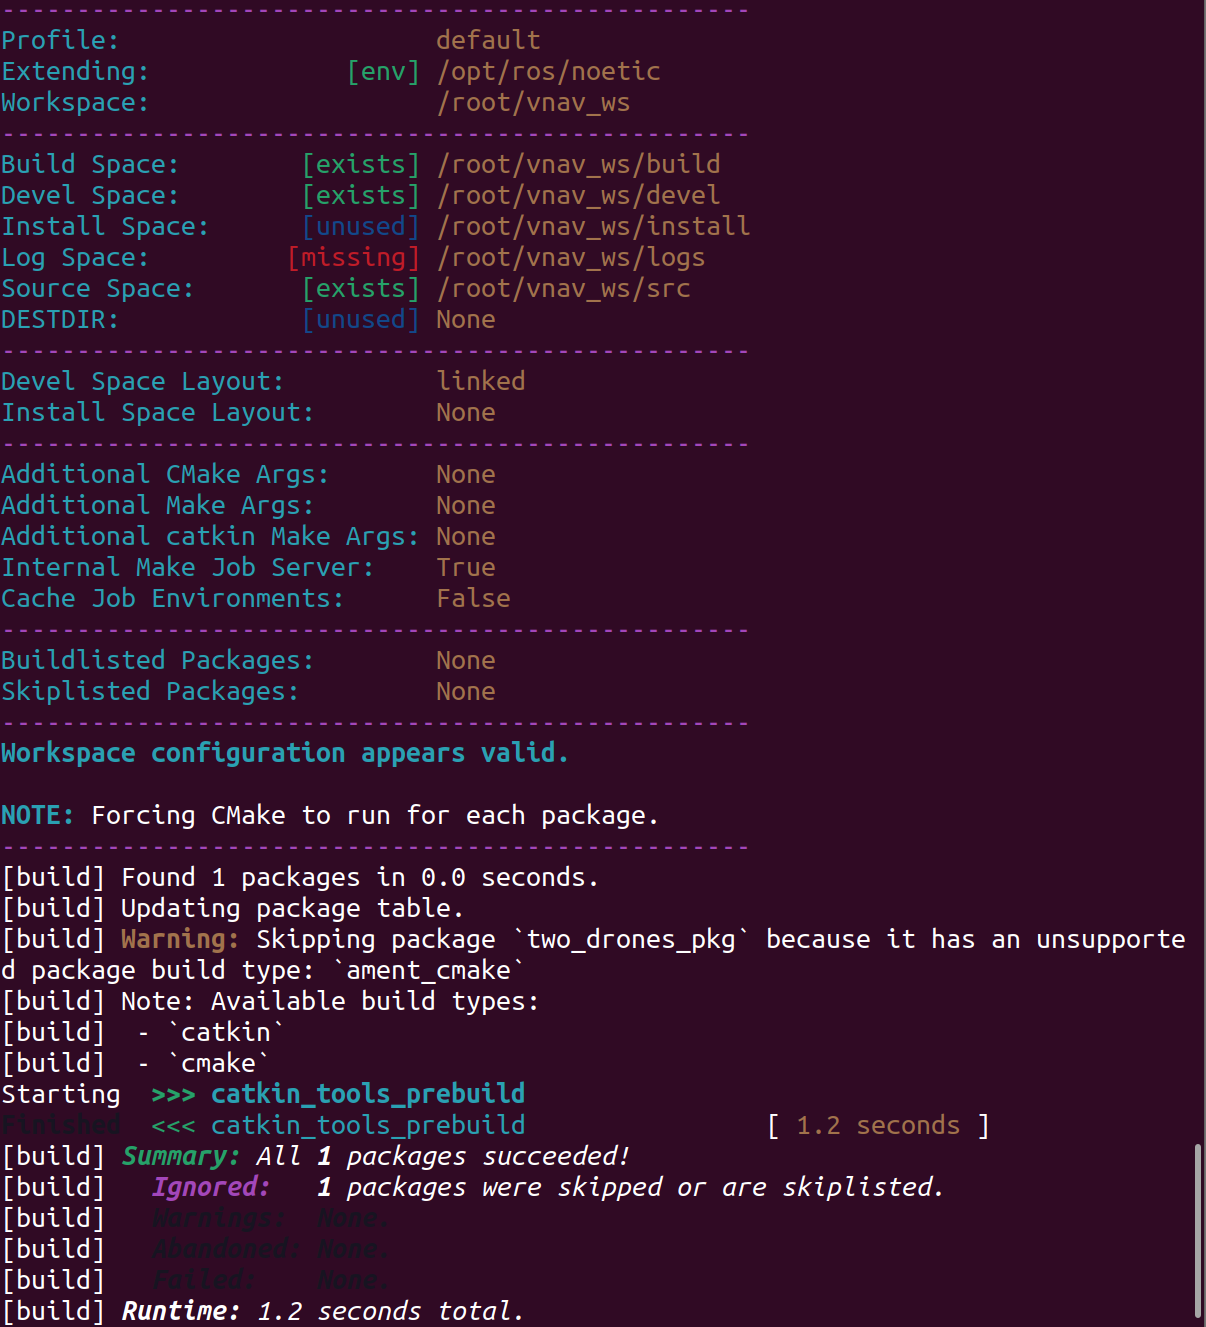
\includegraphics[width=\columnwidth,keepaspectratio]{06_ros2_build_skipped.png}
\caption{Diagnostic first build: the current ROS2 package was skipped by catkin because of \texttt{ament\_cmake}.}
\label{fig:mismatch}
\end{figure}

\begin{figure}[t]
\centering
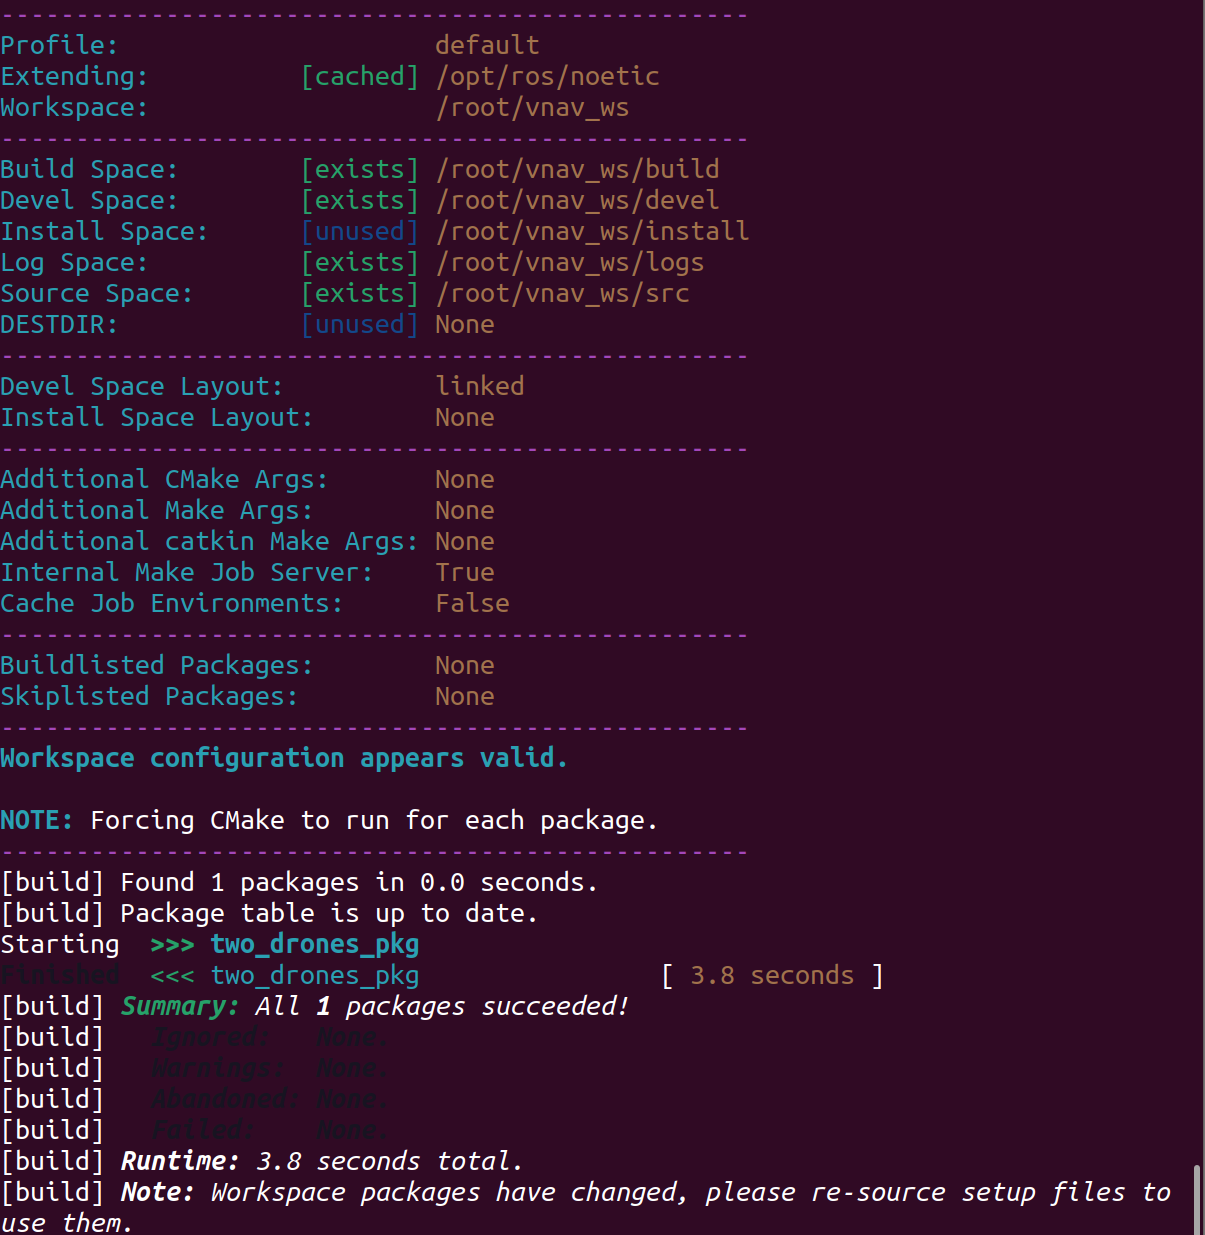
\includegraphics[width=\columnwidth,keepaspectratio]{07_ros1_build_success.png}
\caption{Successful catkin build after switching to the ROS1-compatible commit \texttt{609f31f}.}
\label{fig:ros1build}
\end{figure}

\subsection{Stage 3: Static ROS graph and visualization}
The static scenario was launched with:
\begin{lstlisting}[language=bash]
source /opt/ros/noetic/setup.bash
source /root/vnav_ws/devel/setup.bash
roslaunch two_drones_pkg two_drones.launch static:=True
\end{lstlisting}
The purpose of this stage was to validate the launch file, the package resources, the mesh markers, and the basic TF graph before introducing time-varying motion. The two drones were visible in rViz with \texttt{world} as the fixed frame, and the global status was OK, as shown in Fig.~\ref{fig:staticrviz}.

\begin{figure}[t]
\centering
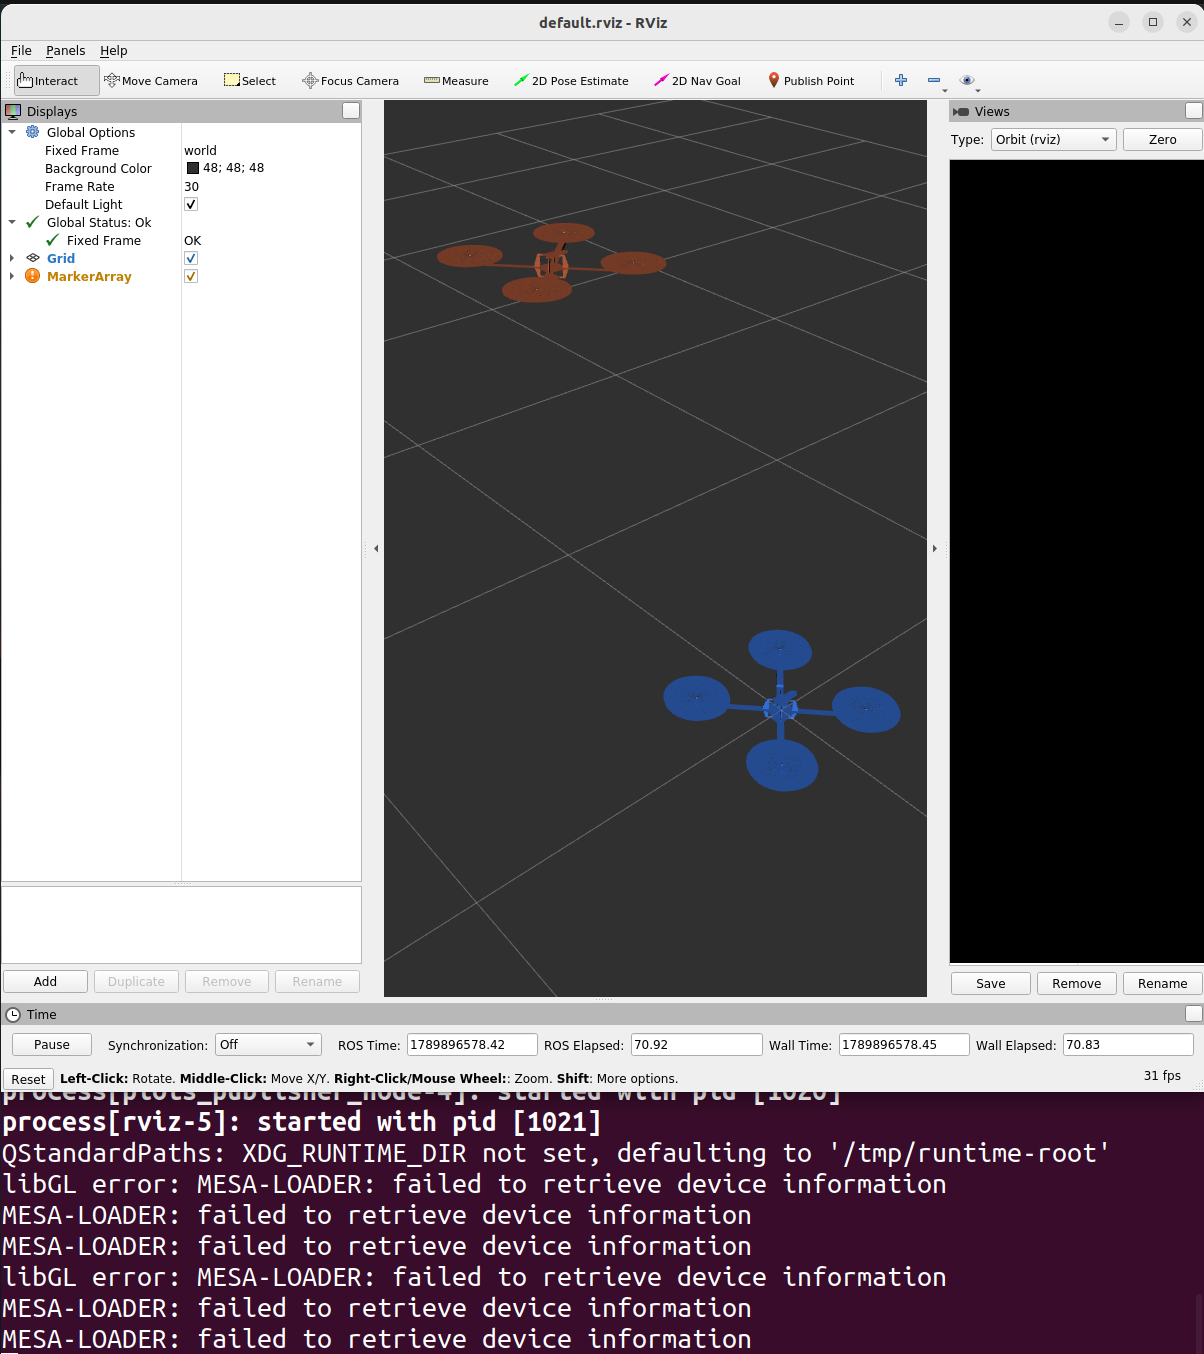
\includegraphics[width=\columnwidth,keepaspectratio]{08_static_rviz.png}
\caption{Static two-drone scene in rViz with the world frame fixed.}
\label{fig:staticrviz}
\end{figure}

The node and topic checks were performed in a second container shell. The recorded nodes included \texttt{/av1broadcaster}, \texttt{/av2broadcaster}, \texttt{/plots\_publisher\_node}, \texttt{/rosout}, and \texttt{/rviz}. The recorded topics included \texttt{/tf}, \texttt{/tf\_static}, \texttt{/visuals}, and standard rViz topics. Figure~\ref{fig:nodes} shows the terminal output, while Fig.~\ref{fig:rqt} shows the graph-level relationship between the broadcasters and the plotting node.

\begin{figure}[t]
\centering
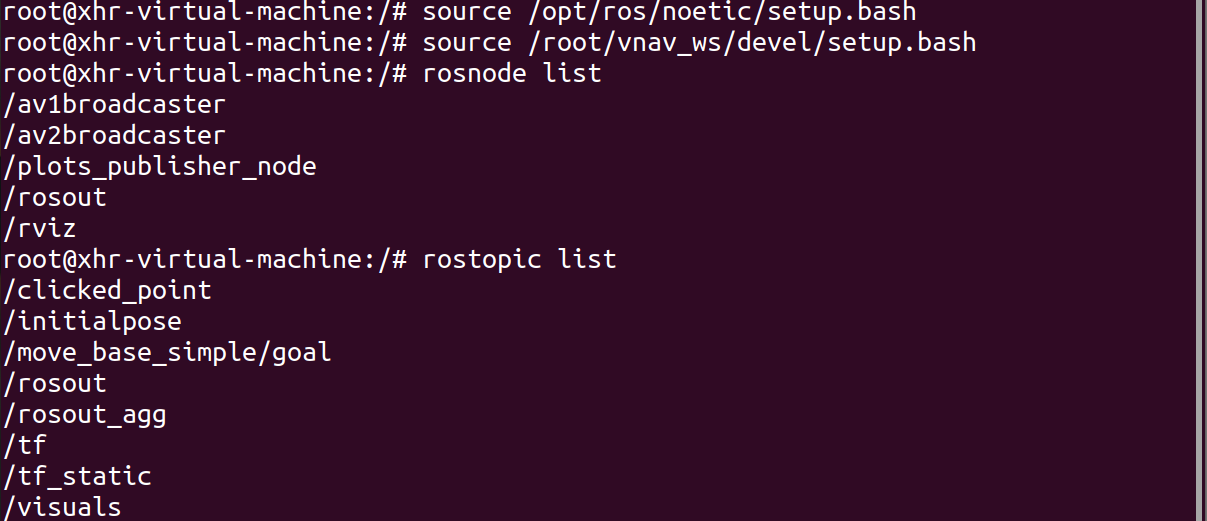
\includegraphics[width=\columnwidth,keepaspectratio]{09_nodes_topics.png}
\caption{Recorded ROS node and topic lists in the static scenario.}
\label{fig:nodes}
\end{figure}

\begin{figure}[t]
\centering
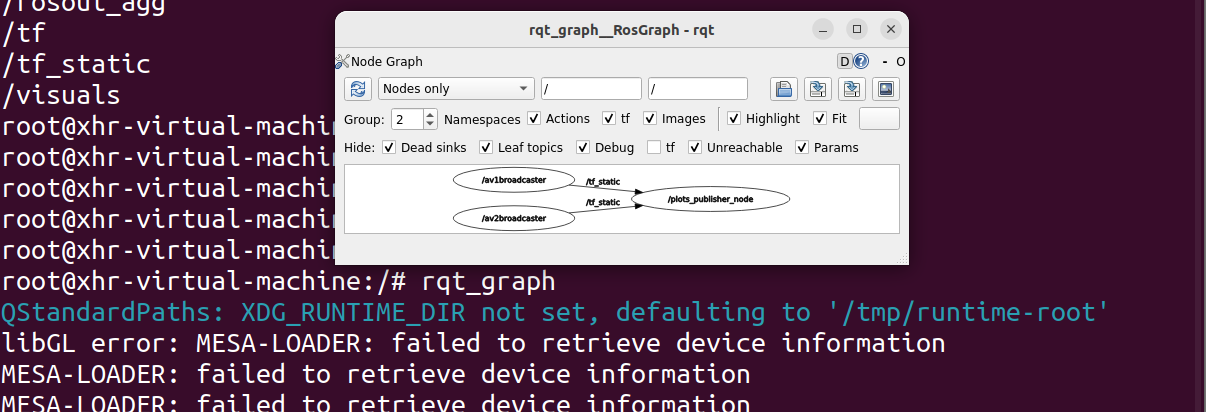
\includegraphics[width=\columnwidth,keepaspectratio]{10_rqt_graph.png}
\caption{rqt\_graph view showing the two broadcasters and the plotting node.}
\label{fig:rqt}
\end{figure}

\subsection{Stage 4: Time-varying TF publication}
The first implementation task was to complete \texttt{frames\_publisher\_node.cpp}. The node runs a 50 Hz timer. At each callback it computes elapsed time, constructs two \texttt{geometry\_msgs/TransformStamped} messages, sets the frame names and translations, computes AV1's yaw quaternion, and broadcasts both transforms.

The input motion specification was:
\begin{align}
o_1^w(t) &= [\cos t,\ \sin t,\ 0]^T,\\
o_2^w(t) &= [\sin t,\ 0,\ \cos(2t)]^T.
\end{align}
The AV1 orientation uses \texttt{setRPY(0,0,t)}, which makes its \(y\)-axis tangent to its circular trajectory while keeping its \(z\)-axis parallel to the world \(z\)-axis. The successful build of this implementation is shown in Fig.~\ref{fig:framesbuild}.

\begin{figure}[t]
\centering
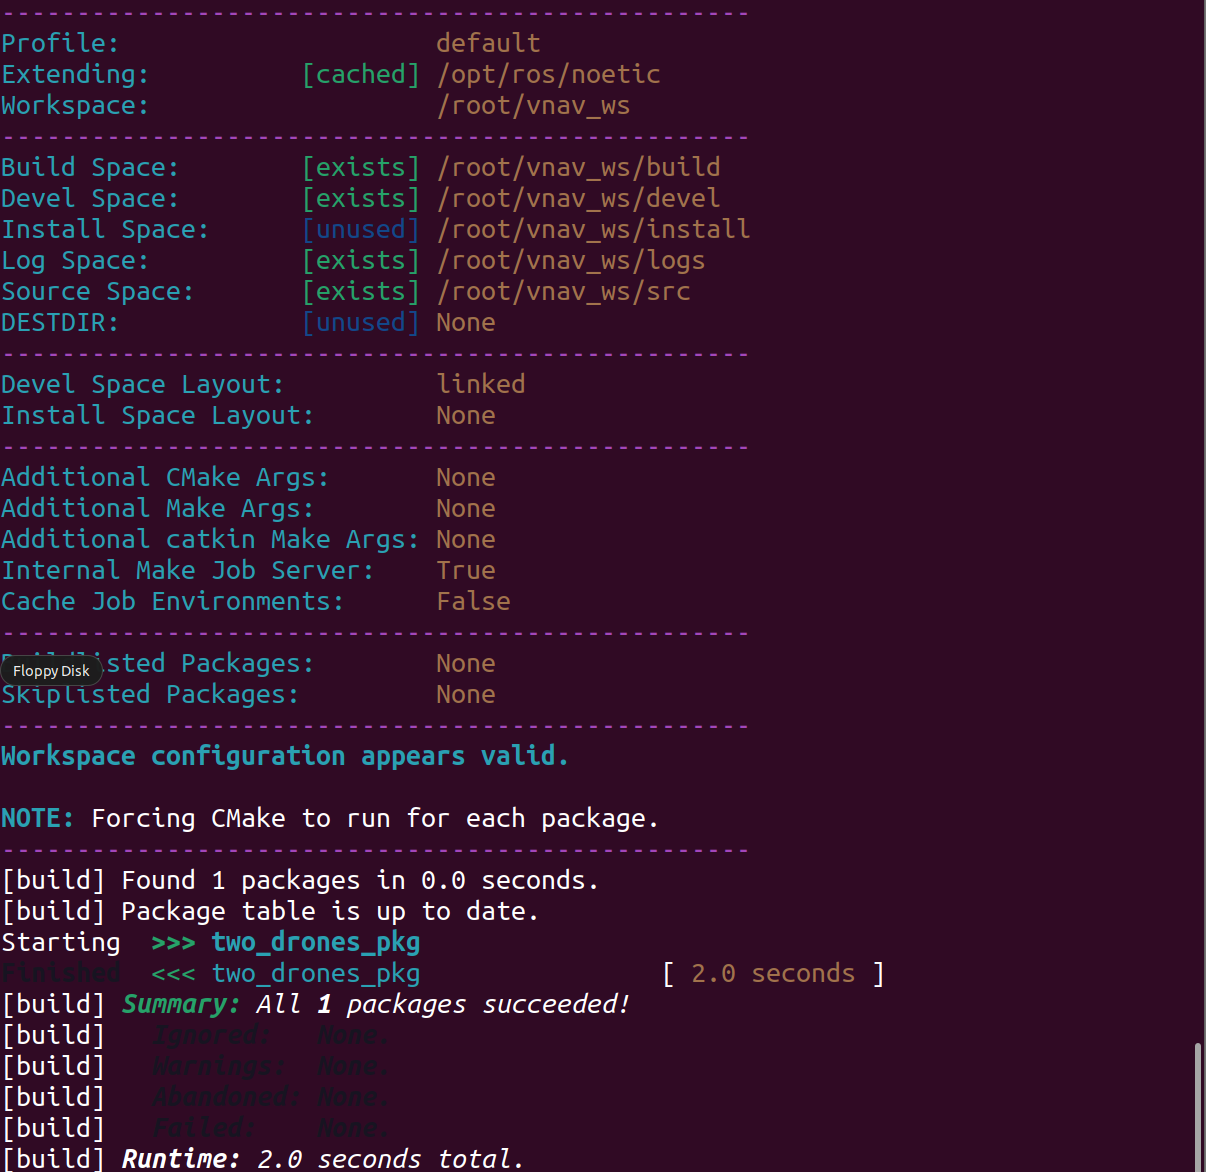
\includegraphics[width=\columnwidth,keepaspectratio]{11_frames_build_success.png}
\caption{Successful build after implementing the time-varying TF broadcaster.}
\label{fig:framesbuild}
\end{figure}

\subsection{Stage 5: Dynamic visualization and relative transform lookup}
The static launch was stopped and the non-static launch was started without the \texttt{static:=True} argument. Two screenshots taken at different times show that the drones changed position, as illustrated in Figs.~\ref{fig:moving1} and \ref{fig:moving2}. This is runtime evidence for the simulated visualization, not evidence of a physical UAV.

\begin{figure}[t]
\centering
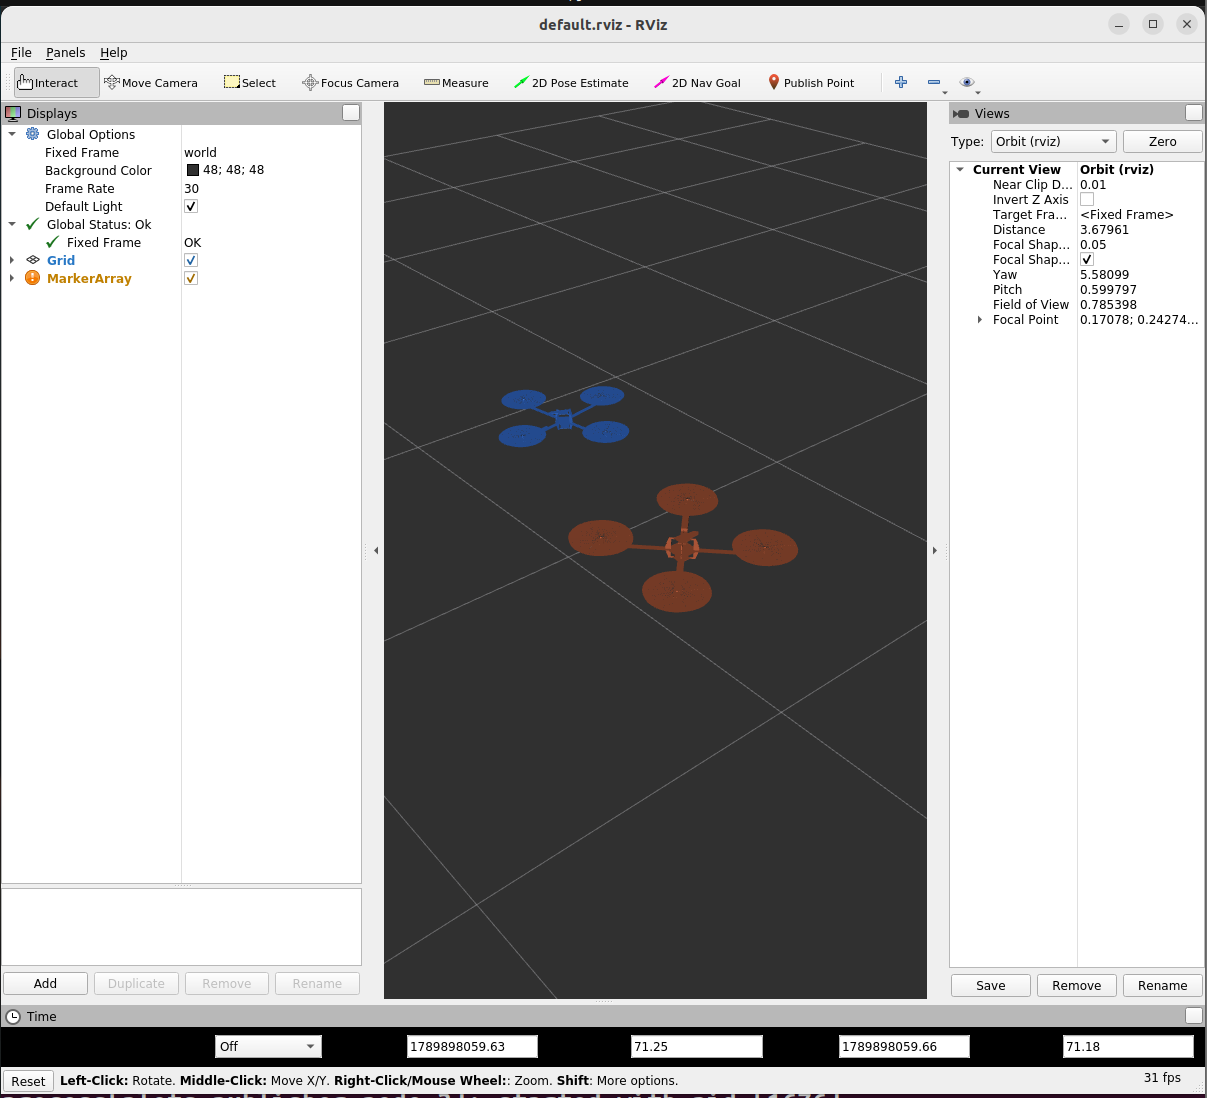
\includegraphics[width=\columnwidth,keepaspectratio]{12_moving_rviz_1.png}
\caption{First recorded view of the moving two-drone scene.}
\label{fig:moving1}
\end{figure}

\begin{figure}[t]
\centering
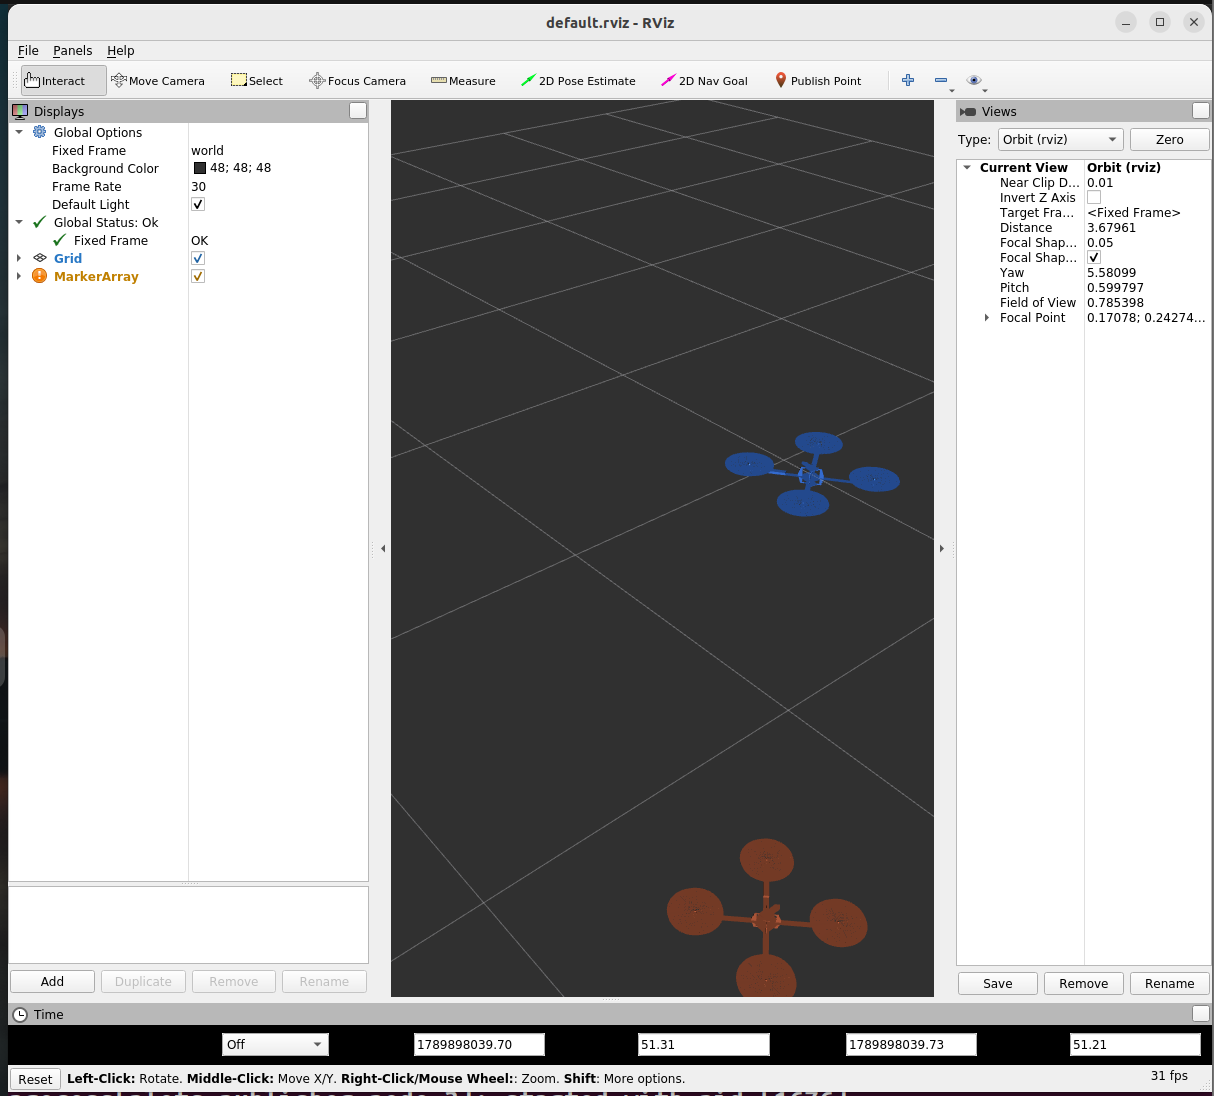
\includegraphics[width=\columnwidth,keepaspectratio]{13_moving_rviz_2.png}
\caption{Second recorded view of the moving two-drone scene at a later time.}
\label{fig:moving2}
\end{figure}

For Deliverable 3, the plotting node was completed with:
\begin{lstlisting}[language=C++]
transform = parent->tf_buffer.lookupTransform(
    ref_frame, dest_frame, ros::Time(0));
\end{lstlisting}
This call requests the latest available transform of the destination frame expressed in the reference frame. After recompilation, the plotting node generated the relative trajectory, and its successful build is recorded in Fig.~\ref{fig:plotsbuild}. Changing rViz's fixed frame from \texttt{world} to \texttt{av1} produced the world-frame circle, the AV2 parabola, and the dashed relative trajectory in Fig.~\ref{fig:av1}.

\begin{figure}[t]
\centering
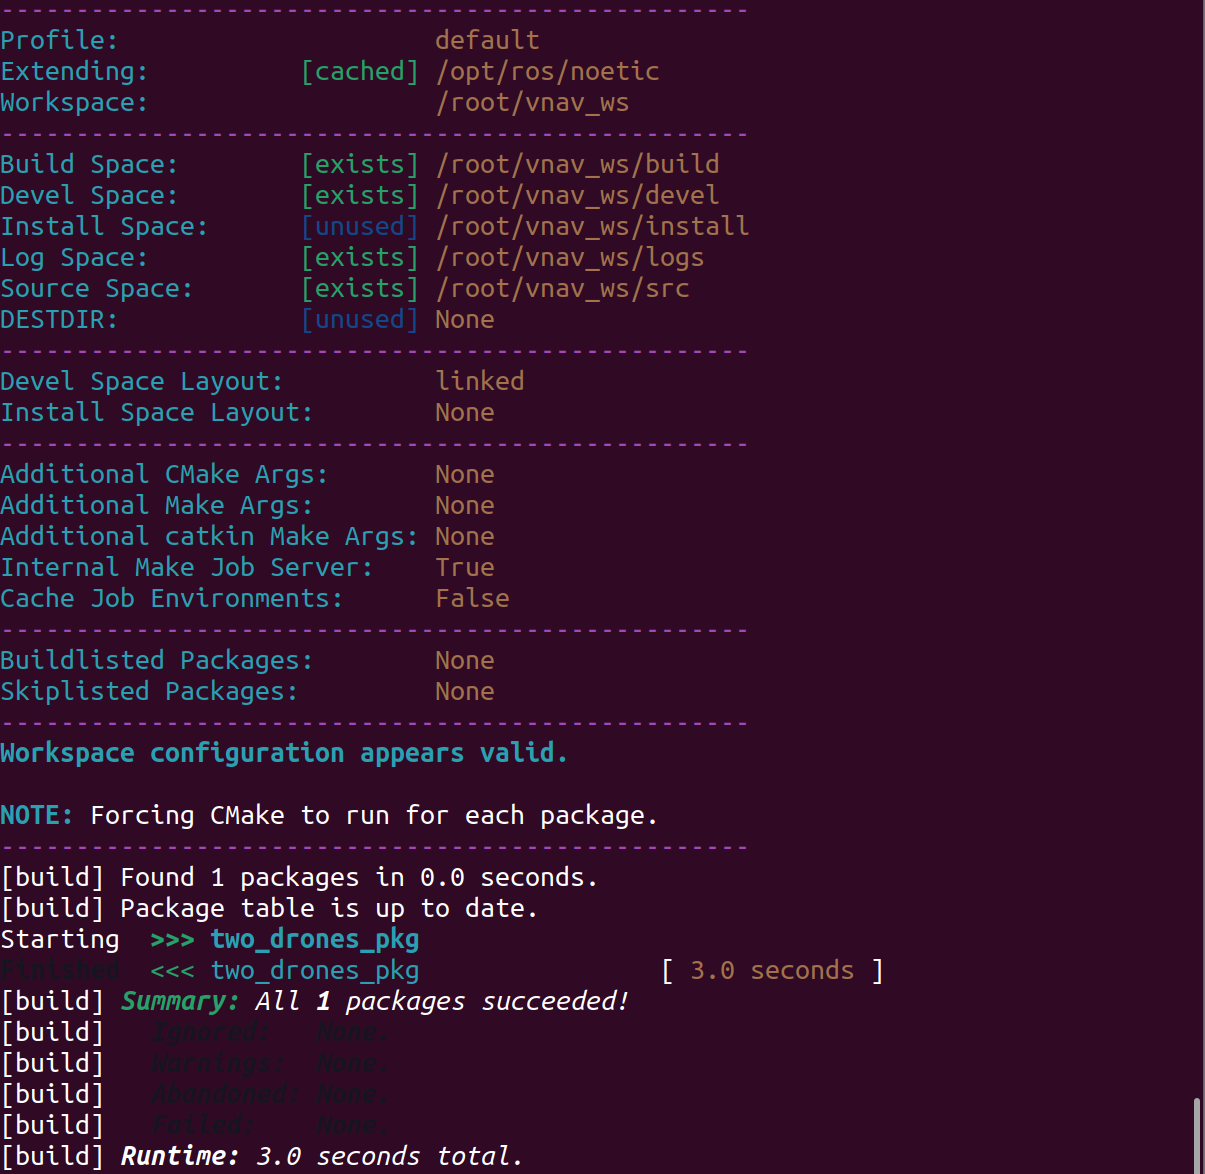
\includegraphics[width=\columnwidth,keepaspectratio]{14_plots_build_success.png}
\caption{Successful build after implementing the relative transform lookup.}
\label{fig:plotsbuild}
\end{figure}

\begin{figure}[t]
\centering
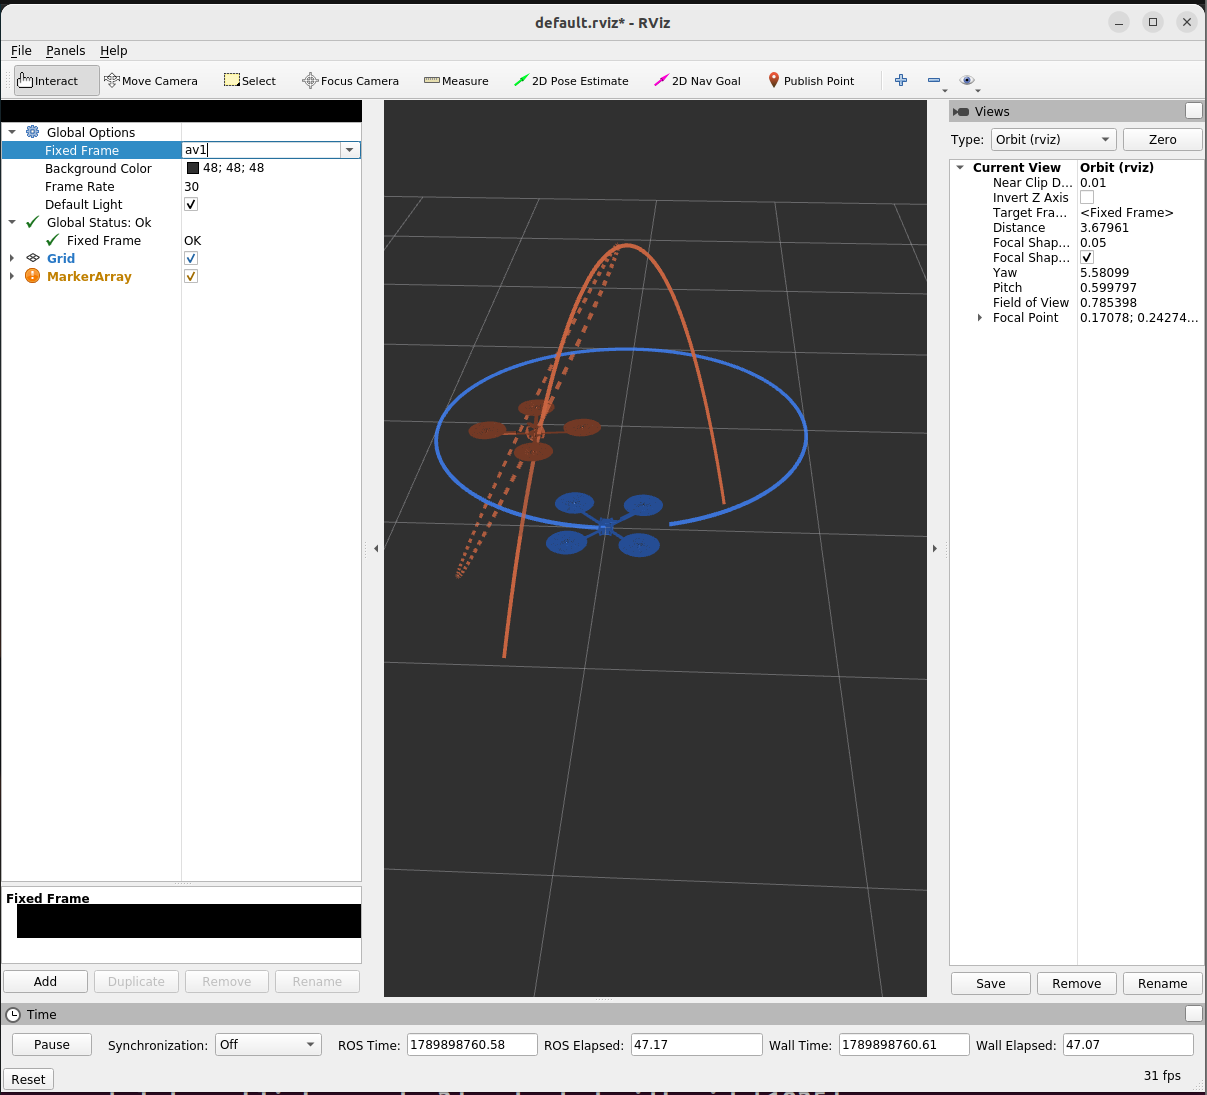
\includegraphics[width=\columnwidth,keepaspectratio]{15_fixed_frame_av1.png}
\caption{rViz with AV1 as the fixed frame, showing the absolute and relative trajectories.}
\label{fig:av1}
\end{figure}

\subsection{Stage 6: turtlesim and Twist-based motion control}
The remaining course tasks were completed with the ROS Noetic \texttt{turtlesim} mobile-robot simulator. This is consistent with the handout's wording that the control exercise may use an unmanned system or mobile robot in simulation. First, \texttt{turtlesim\_node} and \texttt{turtle\_teleop\_key} were launched to verify the standard ROS node and topic path, as shown in Fig.~\ref{fig:turtleteleop}. The subsequent visible motion and command completion are demonstrated separately by the custom controller in Fig.~\ref{fig:turtlecontroller}.

The second control test used a custom Python node named \texttt{turtle\_motion\_controller}. The node published \texttt{geometry\_msgs/Twist} messages to \texttt{/turtle1/cmd\_vel} at 10 Hz. It commanded a forward velocity of 1.0 and an angular velocity of 0.6 for 12 s, then published a zero command to stop the turtle. The terminal recorded both the start and completion messages while the simulator displayed the resulting circular trajectory in Fig.~\ref{fig:turtlecontroller}.

\begin{figure}[t]
\centering
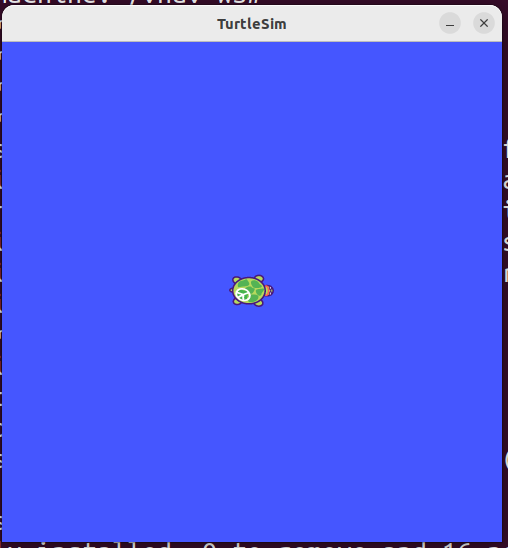
\includegraphics[width=\columnwidth,keepaspectratio]{18_turtlesim_teleop_motion.png}
\caption{Turtlesim and the keyboard teleoperation node launched in the ROS Noetic container.}
\label{fig:turtleteleop}
\end{figure}

\begin{figure}[t]
\centering
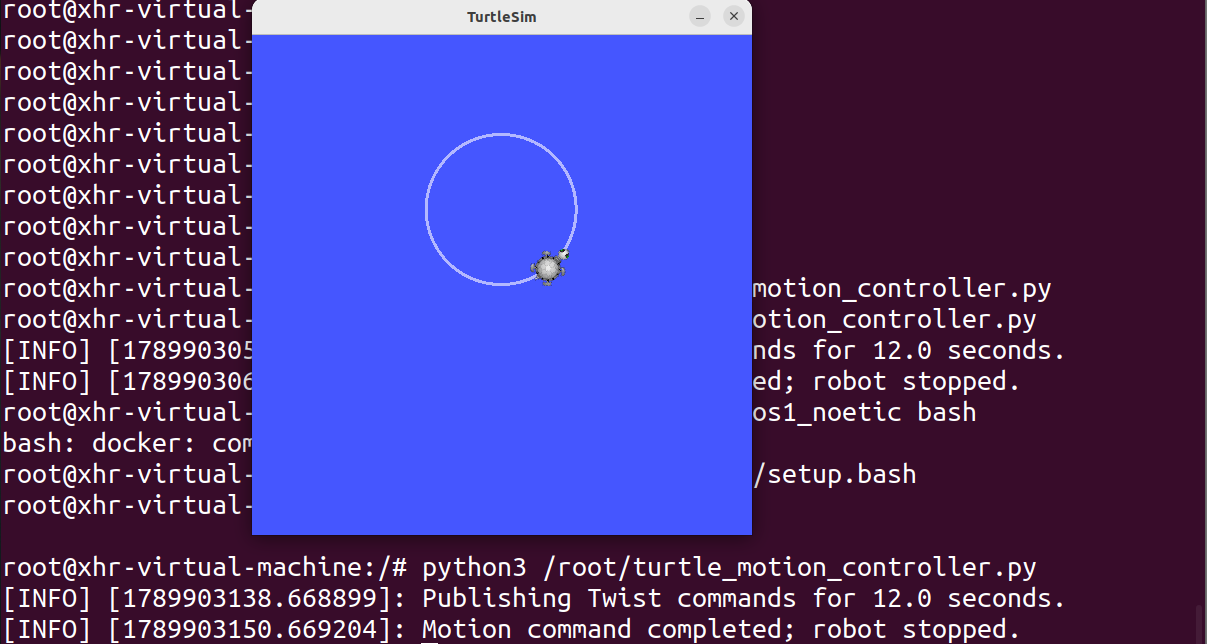
\includegraphics[width=\columnwidth,keepaspectratio]{19_twist_controller_motion.png}
\caption{Custom Twist controller producing a circular turtlesim trajectory and reporting command completion.}
\label{fig:turtlecontroller}
\end{figure}

\subsection{Notion-page verification extensions}
The Notion lab page also specifies several ROS inspection and TF tools. After correcting the container DNS configuration, \texttt{rosdep update} completed and updated the local cache, as shown in Fig.~\ref{fig:rosdep}. The TurtleSim velocity channel was then observed with \texttt{rostopic echo}, and the node/topic relationship was inspected with rqt\_graph in Figs.~\ref{fig:cmdvel} and \ref{fig:turtlegraph}.

The standard \texttt{turtle\_tf} demonstration was launched after installing the missing \texttt{python-is-python3} compatibility command. The two turtle broadcasters, listener, and simulator ran together in Fig.~\ref{fig:tftdemo}. The TF tree, a numerical transform query, and an rViz TF display were then verified in Figs.~\ref{fig:tftree}, \ref{fig:tfecho}, and \ref{fig:rviztf}. These checks complete the previously missing Notion-page tool exercises. The rosdep command was executed as the container root user; its root warning is recorded, while the actual source-cache update succeeded.

\begin{figure}[t]
\centering
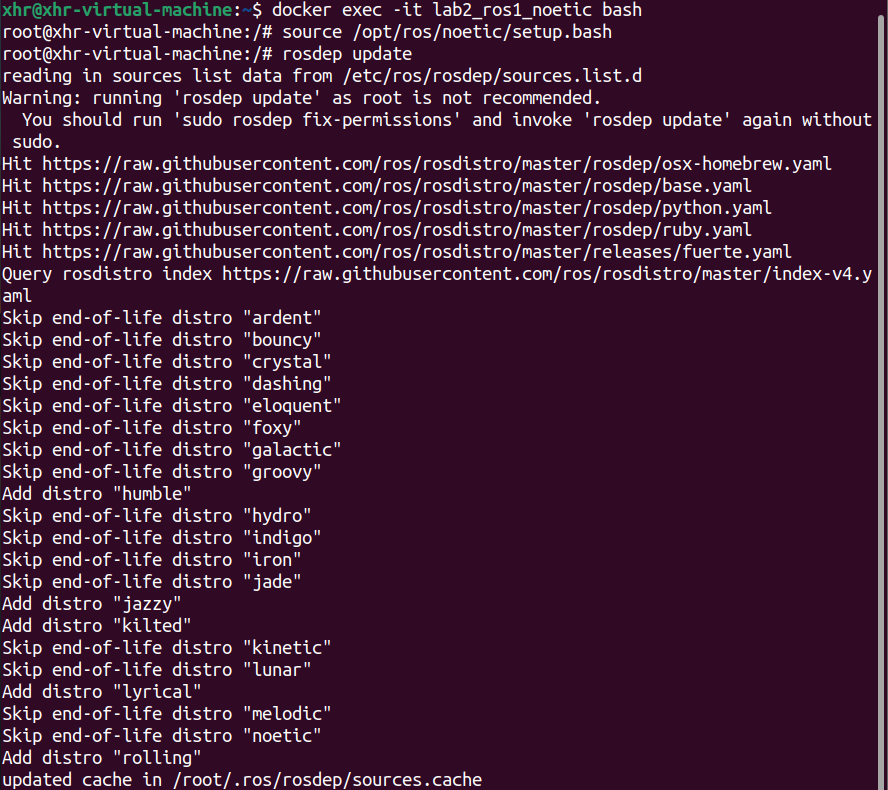
\includegraphics[width=\columnwidth,keepaspectratio]{20_rosdep_update_success.png}
\caption{Successful rosdep source-cache update after repairing container DNS resolution.}
\label{fig:rosdep}
\end{figure}

\begin{figure}[t]
\centering
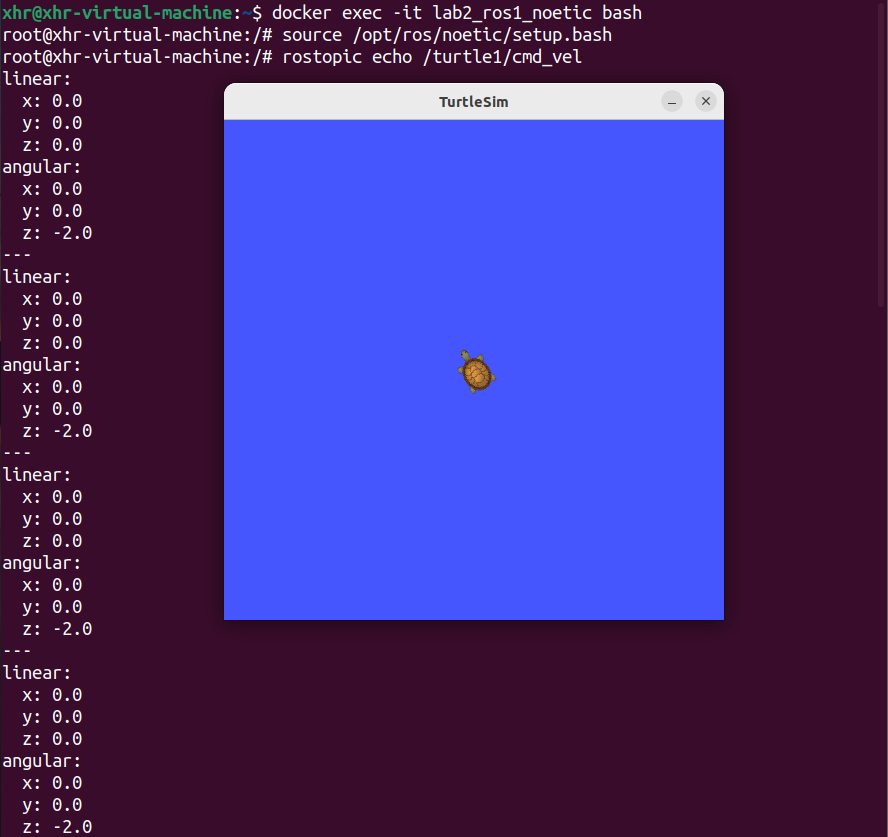
\includegraphics[width=\columnwidth,keepaspectratio]{21_turtle_cmd_vel_echo.png}
\caption{Observed \texttt{/turtle1/cmd\_vel} messages from the teleoperation node.}
\label{fig:cmdvel}
\end{figure}

\begin{figure}[t]
\centering
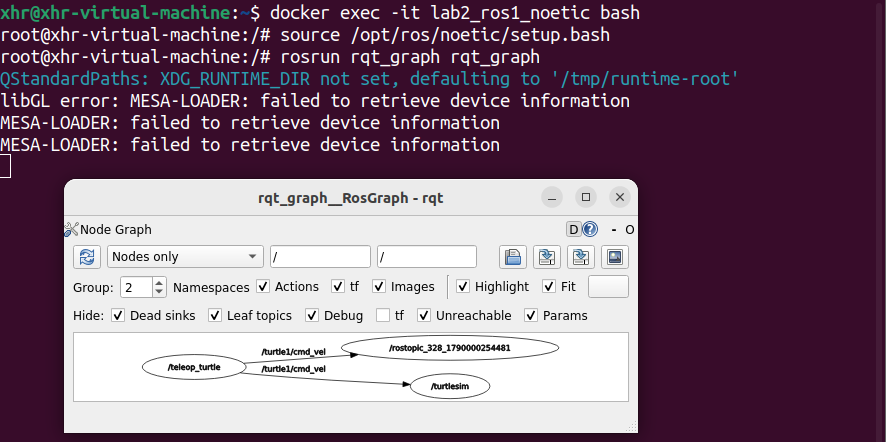
\includegraphics[width=\columnwidth,keepaspectratio]{22_turtlesim_rqt_graph.png}
\caption{rqt\_graph for the TurtleSim teleoperation communication path.}
\label{fig:turtlegraph}
\end{figure}

\begin{figure}[t]
\centering
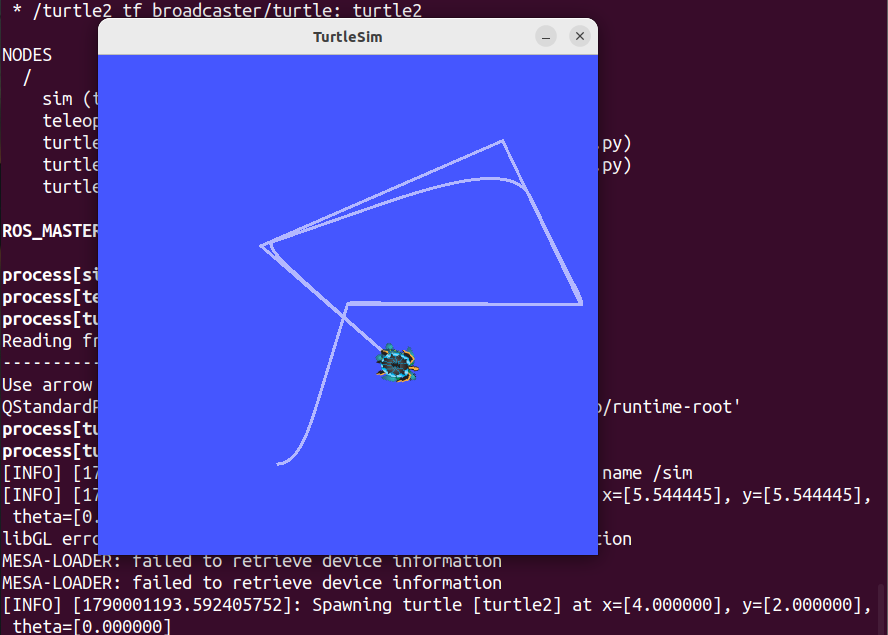
\includegraphics[width=\columnwidth,keepaspectratio]{23_turtle_tf_demo.png}
\caption{The standard turtle TF demonstration with the simulator and TF nodes running.}
\label{fig:tftdemo}
\end{figure}

\begin{figure}[t]
\centering
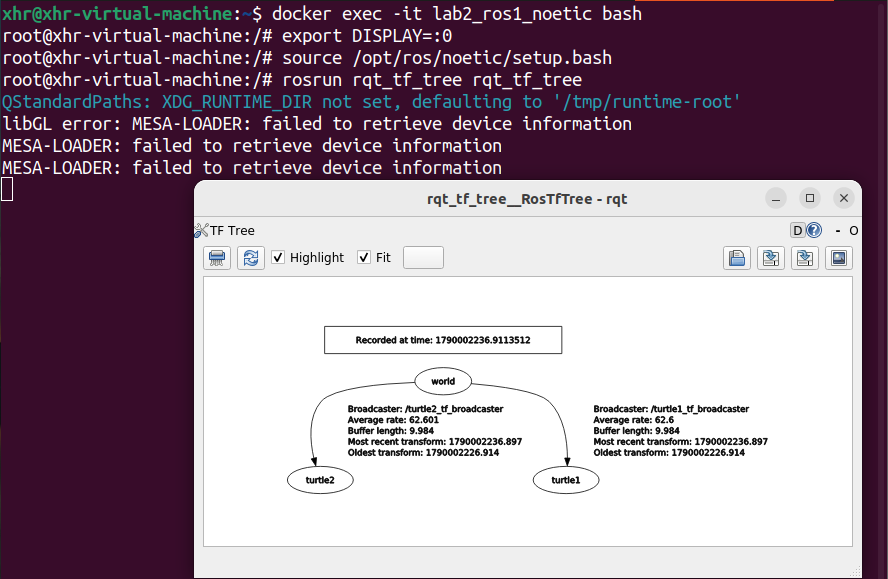
\includegraphics[width=\columnwidth,keepaspectratio]{24_rqt_tf_tree.png}
\caption{rqt\_tf\_tree showing the world, turtle1, and turtle2 frame hierarchy.}
\label{fig:tftree}
\end{figure}

\begin{figure}[t]
\centering
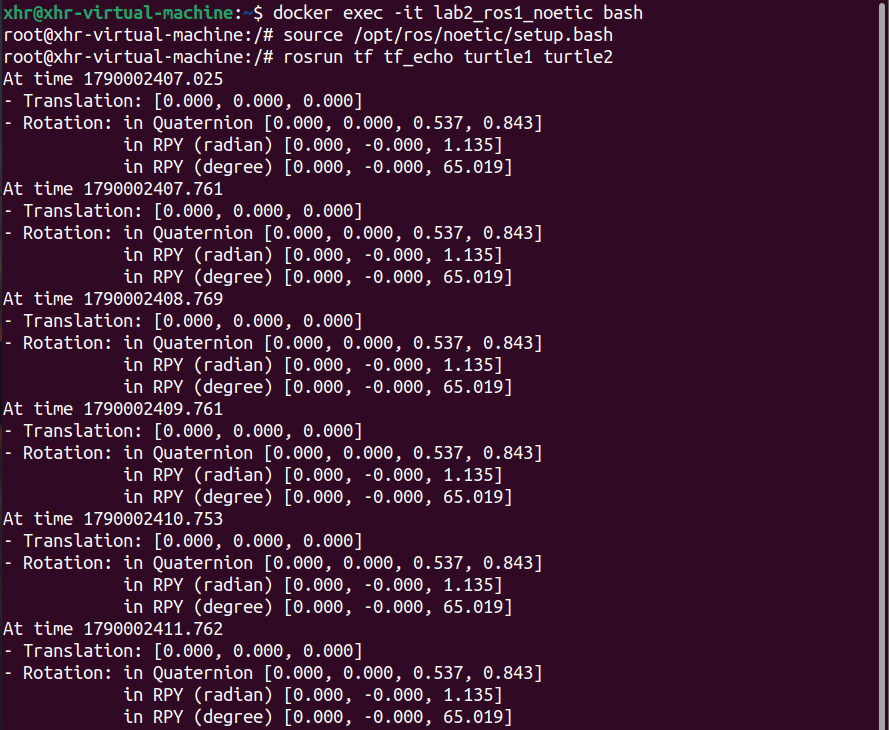
\includegraphics[width=\columnwidth,keepaspectratio]{25_tf_echo_turtle1_turtle2.png}
\caption{Numerical TF query from turtle1 to turtle2, including quaternion and RPY output.}
\label{fig:tfecho}
\end{figure}

\begin{figure}[t]
\centering
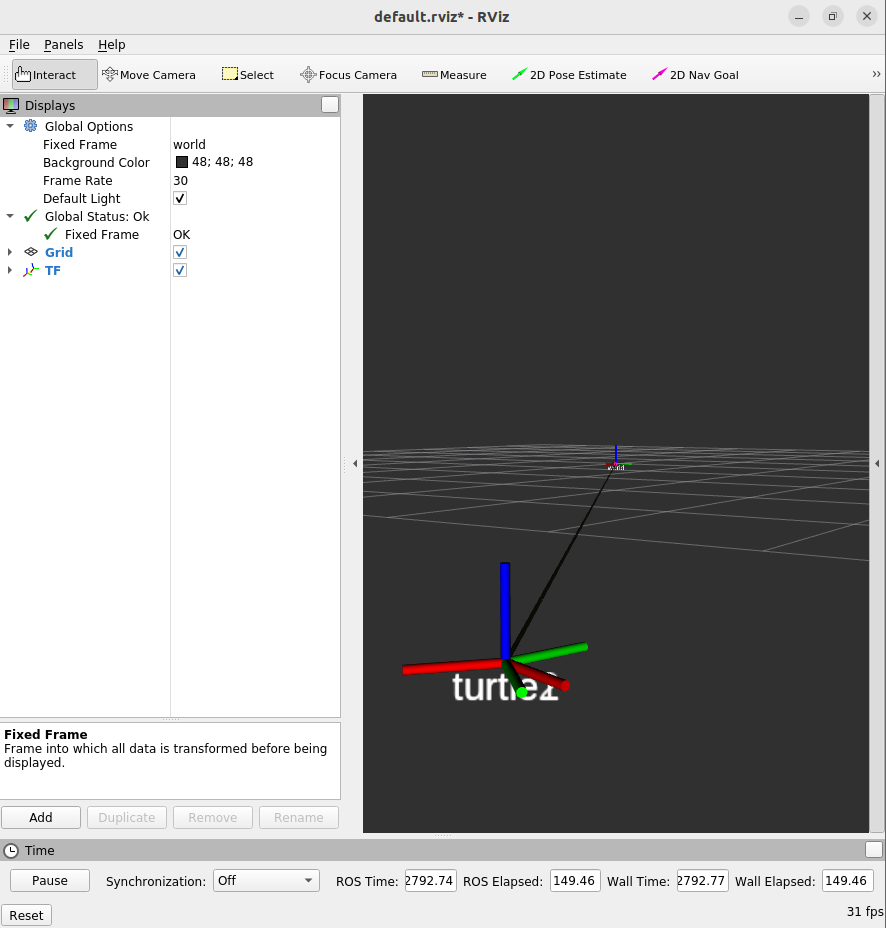
\includegraphics[width=\columnwidth,keepaspectratio]{26_rviz_tf_display.png}
\caption{rViz with the TF display enabled and the world frame selected as fixed frame.}
\label{fig:rviztf}
\end{figure}

\section{IMPLEMENTATION AND EXPERIMENTAL METHOD}
\label{sec:implementation}
\subsection{Package structure and data flow}
The package contains a catkin manifest, a CMake build file, launch and configuration directories, meshes, and C++ source files. The launch file starts the two broadcasters, the plotting node, and rViz. The broadcasters publish TF transforms; the plotting node queries TF and converts the resulting translation into points stored in a bounded trajectory buffer; rViz subscribes to the visual marker output and displays the vehicle meshes and trails.

The data flow is therefore:
\begin{center}
\texttt{time} $\rightarrow$ \texttt{TransformStamped} $\rightarrow$ TF $\rightarrow$ \texttt{lookupTransform} $\rightarrow$ marker trajectory $\rightarrow$ rViz.
\end{center}

\subsection{Transform publisher}
The timer period is 0.02 s, corresponding to 50 Hz. The publisher uses a common timestamp for the two transforms in each callback. AV1 has parent frame \texttt{world}, child frame \texttt{av1}, position \([\cos t,\sin t,0]^T\), and yaw \(t\). AV2 has parent frame \texttt{world}, child frame \texttt{av2}, position \([\sin t,0,\cos(2t)]^T\), and an identity orientation because its orientation is irrelevant to the requested positional analysis.

The key design choice is the AV1 orientation. With yaw \(t\), its body \(y\)-axis is \([-\sin t,\cos t,0]^T\), which is tangent to the circle. This agrees with the problem statement even though the conventional forward axis of a vehicle is often chosen as \(x\).

\subsection{Relative transform lookup}
The lookup uses the TF2 convention \texttt{lookupTransform(target, source, time)}. Passing \texttt{ref\_frame} as the target and \texttt{dest\_frame} as the source returns the destination pose expressed in the reference frame. The call is inside a TF exception handler, so a temporary absence of a transform is reported rather than silently converted into a false trajectory point.

\subsection{Mathematical derivation}
The world-frame AV2 trajectory satisfies \(y=0\), \(x=\sin t\), and \(z=\cos(2t)\). Therefore:
\begin{equation}
z=1-2x^2,
\label{eq:worldparabola}
\end{equation}
which proves that it is a parabola in the world \(x$-$z\) plane.

The AV1-to-world rotation is \(R_1^w=R_z(t)\), so the world-to-AV1 rotation is:
\begin{equation}
R_w^1=R_z(-t)=
\begin{bmatrix}
\cos t&\sin t&0\\
-\sin t&\cos t&0\\
0&0&1
\end{bmatrix}.
\label{eq:rotation}
\end{equation}
Using \(c=\cos t\) and \(s=\sin t\), the relative position is:
\begin{equation}
o_2^1(t)=R_w^1(o_2^w-o_1^w)=
\begin{bmatrix}
cs-1\\-s^2\\\cos(2t)
\end{bmatrix}.
\label{eq:relative}
\end{equation}
Because \(z=1-2s^2=1+2y\), the trajectory lies on:
\begin{equation}
z-2y=1.
\label{eq:plane}
\end{equation}

The center of the curve is \(p=[-1,-1/2,0]^T\). An orthonormal basis for the plane is:
\begin{equation}
e_x=[1,0,0]^T,\qquad e_y=\frac{1}{\sqrt{5}}[0,1,2]^T.
\end{equation}
The centered coordinates are:
\begin{align}
x_p&=\frac{1}{2}\sin(2t),\\
y_p&=\frac{\sqrt{5}}{2}\cos(2t).
\end{align}
Consequently:
\begin{equation}
\frac{x_p^2}{(1/2)^2}+\frac{y_p^2}{(\sqrt{5}/2)^2}=1.
\label{eq:ellipse}
\end{equation}
The semi-axis lengths are therefore \(1/2\) and \(\sqrt{5}/2\), with the longer axis aligned with \(e_y\).

\subsection{Quaternion identities}
For a unit quaternion \(q\), left multiplication by \(q\) and right multiplication by \(q\) preserve the Euclidean norm because quaternion norms multiply. Therefore the matrices \(\Omega_1(q)\) and \(\Omega_2(q)\) are orthogonal. Since \(q^{-1}=[-q_1,-q_2,-q_3,q_4]^T\), their transposes represent multiplication by the inverse and satisfy:
\begin{equation}
\Omega_1(q)^Tq=\Omega_2(q)^Tq=[0,0,0,1]^T.
\end{equation}
Finally, left and right quaternion multiplication commute by associativity:
\begin{equation}
\Omega_1(x)\Omega_2(y)=\Omega_2(y)\Omega_1(x).
\end{equation}
The transpose identity follows because \(\Omega_2(y)^T=\Omega_2(\bar y)\), where \(\bar y\) is the quaternion conjugate.

\subsection{Optional Deliverable 6: intrinsic and extrinsic rotations}
Let \(R_0\), \(R_1\), and \(R_2\) denote the rotations listed in the optional exercise. For the extrinsic interpretation, all rotations are about fixed world axes. Applying \(R_0\), then \(R_1\), then \(R_2\) gives
\begin{equation}
R_{\mathrm{ext}}=R_2R_1R_0.
\label{eq:extrinsic}
\end{equation}
For the intrinsic interpretation, the order is reversed. Starting with the body frame, apply the local rotations \(R_2\), then \(R_1\), then \(R_0\). A local rotation post-multiplies the current orientation, so
\begin{equation}
R_{\mathrm{int}}=I R_2 R_1 R_0=R_2R_1R_0=R_{\mathrm{ext}}.
\label{eq:intrinsic}
\end{equation}
Thus fixed-axis rotations pre-multiply in the listed order, whereas body-axis rotations post-multiply in the reverse order, producing the same final matrix.

For the numerical sequence in the handout,
\begin{equation}
R_0=R_x(90^\circ),\quad R_1=R_y(180^\circ),\quad R_2=R_x(-30^\circ).
\end{equation}
The common final orientation is
\begin{equation}
R_2R_1R_0=
\begin{bmatrix}
-1&0&0\\
0&-1/2&-\sqrt{3}/2\\
0&-\sqrt{3}/2&1/2
\end{bmatrix}.
\label{eq:rotation_equivalence_result}
\end{equation}
The optional deliverable is therefore completed analytically; it does not require an additional runtime experiment.

\section{RESULTS}
\label{sec:results}
The actual results are summarized in Table~\ref{tab:results}. The table distinguishes compilation, visualization, and mathematical verification; no unsupported physical-robot result is included.

\begin{table}[t]
\caption{Verified Lab2 results.}
\label{tab:results}
\centering
\footnotesize
\setlength{\tabcolsep}{2pt}
\begin{tabular}{p{0.31\columnwidth}p{0.23\columnwidth}p{0.34\columnwidth}}
\toprule
Check & Status & Recorded result \\
\midrule
Docker daemon access & Passed & \texttt{docker ps} ran without permission error \\
ROS environment & Passed & \texttt{rosversion -d}: \texttt{noetic} \\
Workspace initialization & Passed & Catkin configuration reported valid \\
ROS1 package build & Passed & One package succeeded; none ignored or failed \\
Static rViz scene & Passed & Two drone models and global status OK \\
Node/topic inspection & Passed & Nodes and TF topics listed; rqt graph displayed \\
Dynamic scene & Passed & Two time-separated rViz views showed changed positions \\
Relative-frame view & Passed & Fixed frame \texttt{av1}; circle, parabola, and dashed relative path visible \\
Turtlesim teleoperation & Passed & Turtlesim and the keyboard teleoperation endpoint launched \\
Twist motion controller & Passed & A custom ROS node published 12 s of velocity commands and then stopped \\
Intrinsic/extrinsic rotation proof & Passed & Matrix products agreed; final orientation given by Eq.~(15) \\
Physical execution & Not performed & No physical UAV or robot was connected \\
\bottomrule
\end{tabular}
\end{table}

The evidence also records the package-version issue. The current repository tip was not silently treated as ROS1: it was identified as an \texttt{ament\_cmake} package and was skipped by catkin. The successful result was obtained only after selecting the historical ROS1 commit \texttt{609f31f}. This distinction is important because a superficially successful catkin command can still mean that a package was ignored.

\section{EVIDENCE AND VERIFICATION}
\label{sec:evidence}
Table~\ref{tab:evidence} establishes the required requirement--operation--result--evidence mapping. The figure paths are relative to the report's \texttt{figures/} directory, and the source paths are relative to the report's \texttt{code/} directory.

\begin{table*}[t]
\caption{Requirement, operation, result, and evidence mapping.}
\label{tab:evidence}
\centering
\footnotesize
\setlength{\tabcolsep}{2pt}
\begin{tabular}{p{0.22\textwidth}p{0.30\textwidth}p{0.25\textwidth}p{0.15\textwidth}}
\toprule
Requirement & Operation & Verified result & Evidence \\
\midrule
Install usable ROS environment & Install Docker, pull Noetic image, source ROS & Noetic container available on Ubuntu 22.04 host & Figs.~\ref{fig:docker}--\ref{fig:rosworkspace} \\
Create and build workspace & Initialize catkin and build ROS1 package & One package succeeded; no ignored or failed packages & Figs.~\ref{fig:package}, \ref{fig:ros1build} \\
Inspect ROS graph & Run \texttt{rosnode list}, \texttt{rostopic list}, and rqt\_graph & Broadcasters, plotting node, TF topics, and graph edges observed & Figs.~\ref{fig:nodes} and \ref{fig:rqt} \\
Publish transforms & Complete the 50 Hz publisher and rebuild & \texttt{world->av1} and \texttt{world->av2} visualized & Fig.~\ref{fig:framesbuild}; code attachment \\
Query relative transform & Complete TF2 lookup and rebuild & Relative path visible in AV1 frame & Figs.~\ref{fig:plotsbuild} and \ref{fig:av1}; code attachment \\
Verify ROS mobile-robot control & Launch turtlesim and teleoperation & Turtlesim and teleoperation endpoint launched & Fig.~\ref{fig:turtleteleop} \\
Publish motion commands & Run the custom Twist controller & Circular trace and stop message recorded & Fig.~\ref{fig:turtlecontroller}; controller code \\
Analyze geometry & Derive position, plane, ellipse, and quaternion properties & Equations~(1)--(7) and quaternion identities & Sec.~\ref{sec:implementation} \\
Prove rotation equivalence & Reverse intrinsic order and compare matrix products & Equations~(13)--(15) agree & Sec.~\ref{sec:implementation} \\
Update rosdep cache & Run \texttt{rosdep update} after DNS repair & Source cache updated successfully & Fig.~\ref{fig:rosdep} \\
Inspect TurtleSim topic graph & Echo \texttt{/turtle1/cmd\_vel} and run rqt\_graph & Velocity messages and publisher/subscriber graph observed & Figs.~\ref{fig:cmdvel} and \ref{fig:turtlegraph} \\
Inspect TF tools & Run turtle TF demo, rqt\_tf\_tree, tf\_echo, and rViz TF & Frame tree, numerical transform, and TF display verified & Figs.~\ref{fig:tftdemo}--\ref{fig:rviztf} \\
\bottomrule
\end{tabular}
\end{table*}

The screenshots are evidence rather than decoration. The Docker screenshots establish host/container setup, the terminal screenshots establish commands and build status, the rViz screenshots establish visualization output, and the rqt graph establishes the ROS communication structure. The screenshots do not prove a physical robot experiment, sensor calibration, timing accuracy, or hardware safety; those items were outside the recorded scope.

\section{DISCUSSION}
\label{sec:discussion}
The results agree with the expected behavior. The static launch produced the two vehicle models and a valid TF visualization. The dynamic launch produced time-separated positions, and changing the fixed frame to AV1 revealed the predicted geometric relationship. The dashed relative path in Fig.~\ref{fig:av1} is consistent with the derived planar ellipse.

The most important implementation detail was the orientation of AV1. A translation-only implementation could still show a circular AV1 path and a moving AV2, but it would produce an incorrect relative trajectory because the body frame would not rotate with the vehicle. The use of yaw \(t\) makes the body \(y\)-axis tangent to the circular path and is therefore necessary for the plane and ellipse derivations.

The most important environment issue was the mismatch between the current repository tip and the older ROS1 exercise. The first catkin invocation reported a successful command overall but explicitly skipped the package because its build type was \texttt{ament\_cmake}. Treating that output as a real package build would have produced an incorrect completion claim. Full history inspection and the switch to \texttt{609f31f} resolved the issue.

The additional turtlesim tests completed the previously missing command-to-motion portion of the handout. They verify a ROS mobile-robot simulation and the \texttt{Twist} interface, but they do not constitute a physical UAV test. The controller's fixed duration and constant velocities make the result easy to repeat, while the absence of a recorded quantitative odometry comparison limits the claim to successful visible motion and command completion.

The experiment is reproducible at the software-visualization level using the recorded host/container arrangement, the ROS1 commit, the workspace commands, and the included screenshots. Exact reproduction of the rViz camera view may vary because the screenshots record interactive camera state, and the report does not include the complete original container filesystem. No physical hardware test, quantitative timing benchmark, or independent numerical comparison against logged trajectory data was recorded. Those are limitations, not missing claims to be filled by assumption.

\section{PERSONAL REFLECTION AND ANALYSIS}
\label{sec:reflection}
The main lesson was that an experiment is a chain of verified states rather than a sequence of commands. The Docker installation was not considered complete until the daemon was reachable without a permission error. The ROS installation was not considered complete until the container returned \texttt{noetic}. The first catkin command was not considered a package build because the package was skipped, even though catkin itself returned a summary containing no failed jobs.

The turtlesim extension made the ROS communication path concrete: a keyboard node and a custom controller both publish to a velocity topic, while the simulator turns those messages into motion. This separated the generic ROS command-to-motion workflow from the more specialized TF trajectory exercise. It also showed why a running ROS master and a running consumer node must be checked separately; a controller can publish successfully while no visible motion occurs if the simulator has already been closed.

The code exercise clarified the relationship between motion equations and coordinate-frame conventions. The formula \([\cos t,\sin t,0]^T\) defines only the origin trajectory; the orientation determines how the same physical motion is represented from the vehicle frame. The TF lookup direction is similarly not a naming detail. Swapping the target and source frames would change the meaning of the returned transform and could produce a visually plausible but mathematically different curve.

The most transferable practice was preserving diagnostic evidence. The skipped ROS2 build was not deleted from the evidence set, because it explains why a historical checkout was required. In a later robotics project, the same approach can prevent a build log, launch file, or installed package from being mistaken for proof that the intended code actually ran.

If the experiment were repeated, I would add an automated numerical check that samples \(o_2^1(t)\) and evaluates the residuals of \(z-2y-1\) and the ellipse equation. I would also record the complete container image digest, the exact package tree, and a clean rebuild from an exported archive. These additions would strengthen reproducibility beyond the current visual and compile evidence.

\balance
\section{CONCLUSIONS}
\label{sec:conclusion}
The Lab2 objectives were achieved for the recorded software-in-the-loop scope. A ROS1 Noetic container was established on the available Ubuntu 22.04 virtual machine, a ROS1-compatible package version was selected, and the catkin workspace compiled successfully. The turtlesim teleoperation and Twist-controller tests completed the command-to-motion exercise. The static and dynamic two-drone scenarios ran in rViz, the ROS graph was inspected, the TF publisher and relative-transform lookup were implemented, and the AV1-fixed visualization displayed the expected trajectories.

The mathematical analysis confirmed that AV2 follows a world-frame parabola, that its AV1-relative trajectory lies on \(z-2y=1\), and that the centered planar trajectory is an ellipse with semi-axis lengths \(1/2\) and \(\sqrt{5}/2\). The final evidence supports compilation and simulated visualization. It does not claim physical-robot execution, hardware validation, or quantitative timing accuracy, because those were not recorded.

\section*{REPRODUCIBILITY STATEMENT}
The following items were reproduced and recorded: Docker daemon access, the ROS Noetic version check, catkin workspace initialization, package compilation at commit \texttt{609f31f}, turtlesim teleoperation, custom Twist-based motion, static and dynamic rViz visualization, node/topic inspection, rqt graph inspection, the AV1-fixed relative trajectory, and the optional intrinsic/extrinsic rotation proof. The mathematical derivations were independently written from the recorded motion equations. Physical execution, hardware timing, odometry-error benchmarking, and a clean rebuild from a newly exported container were not verified and require further testing.

\begin{thebibliography}{99}
\bibitem{handout} Y. Yang, ``LAB2: ROS Installation and Usage,'' course handout, 2025. [Attached PDF.]
\bibitem{mitlab2} MIT VNAV, ``Exercises: Lab 2,'' 2023. [Online]. Available: \url{https://vnav.mit.edu/labs_2023/lab2/exercises.html}
\bibitem{vnavlabs} MIT-SPARK, ``VNAV-labs,'' GitHub repository. [Online]. Available: \url{https://github.com/MIT-SPARK/VNAV-labs}
\bibitem{rosnoetic} Open Robotics, ``ROS Noetic Ninjemys,'' ROS documentation. [Online]. Available: \url{https://wiki.ros.org/noetic}
\bibitem{tf2tutorial} Open Robotics, ``Writing a tf2 listener (C++),'' ROS documentation. [Online]. Available: \url{https://wiki.ros.org/tf2/Tutorials/Writing%20a%20tf2%20listener%20%28C%2B%2B%29}
\bibitem{dockerros} Open Source Robotics Foundation, ``osrf/ros Docker images,'' Docker Hub. [Online]. Available: \url{https://hub.docker.com/r/osrf/ros/tags?name=noetic&page=1}
\end{thebibliography}

\end{document}
